\documentclass[dvipdfmx]{jsarticle}
\usepackage[dvipdfmx]{graphicx}
\usepackage{multicol}
\usepackage{amsthm}
\usepackage[]{multicol}
\usepackage{amsmath}
\usepackage{fancybox}
\usepackage{ascmac}
\usepackage{mathrsfs}
\usepackage{amsfonts}
\usepackage{amssymb}
\usepackage{tikz}
\usepackage{wrapfig}
\usepackage{latexsym}
\usepackage{MnSymbol}
\usetikzlibrary{cd}
\newtheorem*{answer*}{解答}
\newtheorem{prob}{}[]
\newtheorem{definition}[prob]{定義}
\newtheorem{dfn}[prob]{定義}
\newtheorem{theorem}[prob]{定理}
\newtheorem*{lemma*}{補題}
\newtheorem{answer}{解答}
\newtheorem*{proof*}{証明}
\begin{document}


\hskip1zw {\Large Asahi\ Math Contest 002} 
\hskip1zw R3.9.11 第$74$回朝日祭\\  % \hskipは水平方向にスペースを作ります
\rightline {岡山朝日数学同好会}\\
\underline{\hskip2zw年 \hskip2zw 組 \hskip2zw 番\hskip1zw 氏名 \hskip30ex} \\
{\Large{*注意}}\\
\underline{$\binom{n}{k} $で二項係数${}_{n}{\mathrm{C} }_{k}$と同じことを表すものとする.\hskip27zw} 
%大問1
\begin{prob}
  $1$本の道路があり,図$1$のように枝分かれしている.
  枝分かれした道路の先には必ず労働者の家がある.
  いま,この道路のどこかにバス停をひとつ作ることを考える.
  各労働者の家からバス停までの移動距離の合計がもっとも短くなるようにするにはどこにバス停を作ればよいか.
\end{prob} 
\begin{figure}[h]
  \centering
  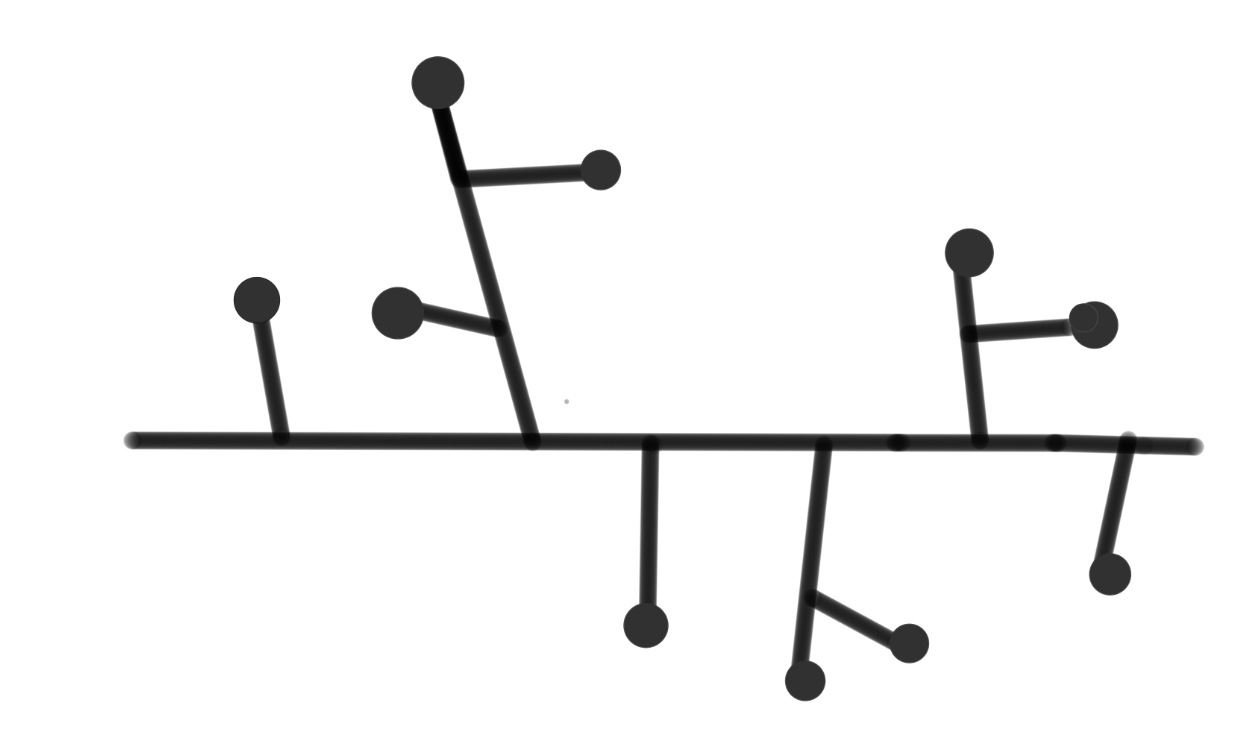
\includegraphics[width=10cm]{AMC002-picture/mathtest3.png}
  \caption {}\label{ex1}
\end{figure}

\vfill
%大問2
\begin{prob}
  数列$\{a_{n}\}$が$a_{1}=3,(2n+1)a_{n+1}=2na_{n}+1$を満たすとき,$a_{n}$を$n$を用いて表せ.
\end{prob}
\vfill

%大問3
\begin{prob}
  $O$を原点とする$xyz$空間座標系において,$xy$平面上の点ではない$2$点$A,B$からそれぞれ$xy$平面へ下ろした垂線の足を$P,Q$とおく.
  $\angle AOP=\alpha ,\angle BOQ=\beta,\angle POQ=\gamma$とするとき,
  $\cos \angle AOB$を$\alpha,\beta,\gamma$を用いて表せ.  
\end{prob}
\vfill

%大問4
\begin{prob}
  $n$を$3$以上の整数とする.$1$辺の長さを$1$とする正$2n$角形の最も短い対角線の長さを$l_{n}$,最も長い対角線の長さを$L_{n}$とする.このとき,以下の級数の収束・発散を判定せよ.また,収束するならばその和を求めよ.
\begin{align*}
  \sum_{n=3}^{\infty}{\frac{1}{l_{n}\cdot L_{n}}}
\end{align*} 
\end{prob}
\vfill

%大問5
\begin{prob}
   $p$を素数とする.このとき,
\begin{align*}
  \sum_{n=1}^{p-1}\binom{p-1}{n}\frac{1}{n^{2p}} 
\end{align*}
  を既約分数で表したとき,分子は$p$で最大何回割り切れるか. 
\end{prob}
\vfill
%大問6
\begin{prob}
  次の値を求めよ.
  \begin{align*}
    \int_{0}^{\frac{1}{\sqrt[3]{2} }}  \frac{\,dx }{\sqrt[3]{1-x^3}}
  \end{align*}
\end{prob}
\vfill

%大問7
\begin{prob}
  $p$を素数,$n,k\in \mathbb{N}$,$m\in \mathbb{N}$を $p$の倍数でない数とする.このとき,
\begin{align*}
  \sum_{i=0}^{n}(-1)^i\binom{n}{i}\binom{p^km+n-i}{p^k-i}
\end{align*}
は$p$で割り切れるか.
\end{prob}
\vfill
%大問8
\begin{prob}
  $xyz$空間座標系において,点$O(0,0,0)$,$P(a,b,c)$を通る直線を軸とする半径$r$の円柱面の方程式を求めよ.
\end{prob}
\vfill
%大問9
\begin{prob}
  空間上に正四面体$OXYZ$がある.点$P$が準格子点であるとは,ある整数$a,b,c$が存在し,
\begin{align*}
  \overrightarrow{OP}=a\overrightarrow{OX}+b\overrightarrow{OY}+c\overrightarrow{OZ}  
\end{align*}
を満たすことをいう.このとき,正多面体に関する次の条件を満たすものを全て挙げよ.
\begin{align*}
  (*)準格子点を結ぶことで作れない.
\end{align*}  
\end{prob}
\vfill
%大問10
\begin{prob}
  領域$0\leq x \leq \frac{\pi}{2}$において,曲線$y=-3\cos x+2$と$2$直線$x=1$,$y=-1$で囲まれた図形の面積を$S_{1}$,
  曲線$y=-4\cos x+2$と$2$直線$x=1$,$y=-2$で囲まれた図形の面積を$S_{2}$,$2$曲線$y=-2\cos x+2$,$y=-4\cos x+2$と$y$軸で囲まれる面積から
  $0\leq x \leq 1$,$-2\leq y\leq 0$の部分を除いた図形の面積を$S_{3}$とする.このとき,$S_{1}$:$\left(S_{2}+S_{3}\right)$を最も簡単な整数比で表せ.
\end{prob}
\vfill
\end{document}


